\documentclass{beamer}

\usepackage{amsmath}
\usepackage{pgfplots}
\usepgfplotslibrary{fillbetween}
\usepackage{minted}
\usepackage[T1]{fontenc}
\usepackage{multicol}
\usepackage{booktabs}

\usecolortheme{rose}

\author{Tom Deakin}
\title{OpenMP for Computational Scientists}
\subtitle{The Pi program}

\begin{document}

\frame{\titlepage}

%-------------------------------------------------------------------------------

\section{Outline}
\begin{frame}
\frametitle{Outline}
\begin{itemize}
  \item Data sharing clauses
  \item The Pi program
  \item Critical regions
  \item Atomics
  \item False sharing issues
  \item Reductions
\end{itemize}
\end{frame}
%-------------------------------------------------------------------------------

\section{Data sharing}
\begin{frame}
\frametitle{Data sharing}
Remember: OpenMP is a \emph{shared} programming model.
By default, all data is available to all threads.

There is a single copy of \emph{shared} data.

You must specify which data should be \emph{private} to each thread.
Each thread then has local (stack) space for each private variable.
Each copy is only visible to its associated thread.
\end{frame}


%-------------------------------------------------------------------------------
\begin{frame}
\frametitle{Variables on the heap}
All data on the heap is shared.
Therefore all the Fortran \mintinline{fortran}|allocatable| data is shared.
You must ensure that different threads do not write to the same element of these arrays.

Setting a data sharing clause on a heap variable only effects the metadata of the variable.
The pointer could be private, but the target will be shared.
\end{frame}

%-------------------------------------------------------------------------------
\section{Data clauses}
\begin{frame}
\frametitle{Data clauses}
\begin{itemize}
  \item \mintinline{fortran}|shared(x)|
    There is one copy of the \mintinline{fortran}|x| variable. The programmer must ensure synchronisation.
  \item \mintinline{fortran}|private(x)|
    Each thread gets its own local \mintinline{fortran}|x| variable. It is not initialised. The value of the original \mintinline{fortran}|x| variable is undefined on region exit.
  \item \mintinline{fortran}|firstprivate(x)|
    Each thread gets its own \mintinline{fortran}|x| variable, and it is initialised to the value of the original variable entering the region.
  \item \mintinline{fortran}|lastprivate(x)|
    Each thread gets its own \mintinline{fortran}|x| variable, and the original variable is updated from the last iteration.
\end{itemize}

There is also the \mintinline{fortran}|threadprivate(x)| directive.
This says to take a copy of the data in \emph{thread local storage} which is persistent across parallel regions.
\end{frame}

%-------------------------------------------------------------------------------
\subsection{Private example}
\begin{frame}[fragile]
\frametitle{Private example}
Simple \mintinline{fortran}|do| loop, which just sets a variable to the iteration number.
Each iteration prints out the current, and next value of \mintinline{fortran}|x|, along with the thread number.
Will see what happens with different data sharing clauses.

\begin{minted}[linenos,breaklines]{fortran}
  !$omp parallel do private(x) / firstprivate(x) / lastprivate(x)
  do i = 1, N
    write (*,"(2X,A,I0,A,I0,A,I0)") "Thread ", omp_get_thread_num(), " setting x=", x, " to ", i
    x = i
  end do
  !$omp end parallel do
\end{minted}
N is set to 10.
\end{frame}

%-------------------------------------------------------------------------------
\begin{frame}[fragile]
\frametitle{Private example}
\begin{minted}{bash}
private:
 before: x=-1
  Thread 1 setting x=0 to 4
  Thread 2 setting x=0 to 7
  Thread 3 setting x=0 to 9
  Thread 0 setting x=0 to 1
  Thread 1 setting x=4 to 5
  Thread 2 setting x=7 to 8
  Thread 3 setting x=9 to 10
  Thread 0 setting x=1 to 2
  Thread 1 setting x=5 to 6
  Thread 0 setting x=2 to 3
 after: x=-1
\end{minted}
Each thread starts with its own \mintinline{fortran}|x|, which set to zero (the default value of an integer in Fortran).
In C, it would probably be filled with garbage.
\end{frame}

%-------------------------------------------------------------------------------
\begin{frame}[fragile]
\frametitle{Private example}
\begin{minted}{bash}
firstprivate:
 before: x=-1
  Thread 3 setting x=-1 to 9
  Thread 2 setting x=-1 to 7
  Thread 1 setting x=-1 to 4
  Thread 0 setting x=-1 to 1
  Thread 3 setting x=9 to 10
  Thread 2 setting x=7 to 8
  Thread 1 setting x=4 to 5
  Thread 0 setting x=1 to 2
  Thread 1 setting x=5 to 6
  Thread 0 setting x=2 to 3
 after: x=-1
\end{minted}
Each thread starts with its own \mintinline{fortran}|x|, which set to the value of \mintinline{fortran}|x| before entering the \mintinline{fortran}|parallel| region, -1.
\end{frame}

%-------------------------------------------------------------------------------
\begin{frame}[fragile]
\frametitle{Private example}
\begin{minted}{bash}
lastprivate:
 before: x=-1
  Thread 3 setting x=3 to 9
  Thread 2 setting x=2 to 7
  Thread 1 setting x=1 to 4
  Thread 3 setting x=9 to 10
  Thread 0 setting x=0 to 1
  Thread 2 setting x=7 to 8
  Thread 1 setting x=4 to 5
  Thread 0 setting x=1 to 2
  Thread 1 setting x=5 to 6
  Thread 0 setting x=2 to 3
 after: x=10
\end{minted}
Each thread starts with its own \mintinline{fortran}|x|, which set to to a garbage value.
On exiting the region, the original \mintinline{fortran}|x| is set to the value of the last iteration of the loop, 10.
\end{frame}

%-------------------------------------------------------------------------------
\section{Default data sharing}
\begin{frame}
\frametitle{Choosing default data sharing}
\begin{alertblock}{Note}
It is especially important to list private variables in Fortran.
All variables are \emph{global} scope so \emph{everything} is shared by default.
In C, local scoping rules makes this easier.
\end{alertblock}

You can force yourself to specify everything manually by using the \mintinline{fortran}|default(none)| attribute.
You can also \mintinline{fortran}|default(private)| or \mintinline{fortran}|default(firstprivate)| to make everything private by default --- this might save a lot of typing in an old code with many temporary variables.

\end{frame}

%-------------------------------------------------------------------------------
\section{Calculating Pi}
\begin{frame}
\frametitle{Integration to calculate Pi}
$$\int_{0}^{1} \frac{4}{1+x^2} dx = \pi$$

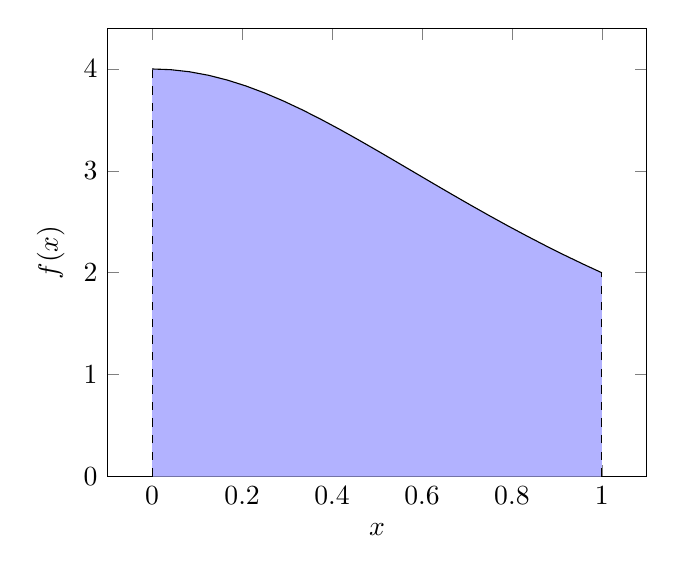
\begin{tikzpicture}
  \begin{axis}[xlabel={$x$},ylabel={$f(x)$},ymin=0]
    \addplot [name path=A, domain=0:1] {4/(1+x*x)};
    \addplot[dashed] coordinates {(0,0) (0,4)};
    \addplot[dashed] coordinates {(1,0) (1,2)};
    \path [name path=axis] (axis cs:0,0) -- (axis cs:1,0);
    \addplot[blue!30] fill between [of=A and axis, domain=0:1];
  \end{axis}
\end{tikzpicture}
\end{frame}

%-------------------------------------------------------------------------------
\begin{frame}
\frametitle{Trapezoidal rule}
Sum the area of the boxes. Choose a small \emph{step} size to generate lots of boxes, and increase accuracy.
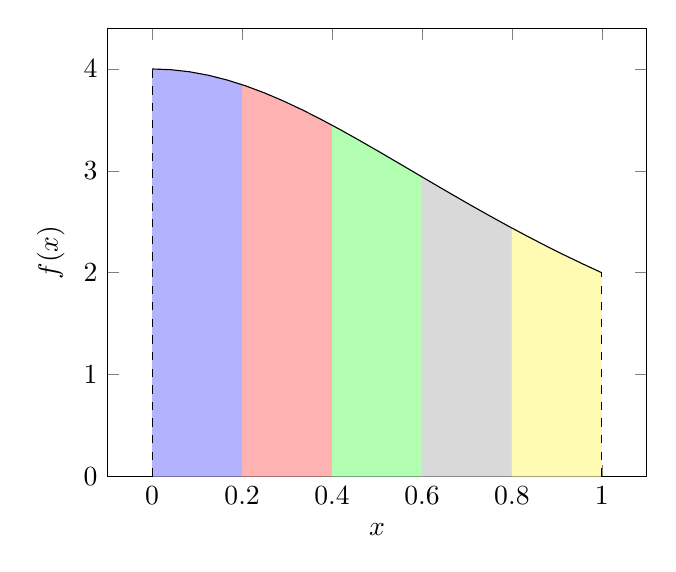
\begin{tikzpicture}
  \begin{axis}[xlabel={$x$},ylabel={$f(x)$},ymin=0]
    \addplot [name path=A, domain=0:1] {4/(1+x*x)};
    \addplot[dashed] coordinates {(0,0) (0,4)};
    \addplot[dashed] coordinates {(1,0) (1,2)};
    \path [name path=axis] (axis cs:0,0) -- (axis cs:1,0);
    \addplot[blue!30] fill between [of=A and axis, soft clip={domain=0:0.2}];
    \addplot[red!30] fill between [of=A and axis, soft clip={domain=0.2:0.4}];
    \addplot[green!30] fill between [of=A and axis, soft clip={domain=0.4:0.6}];
    \addplot[gray!30] fill between [of=A and axis, soft clip={domain=0.6:0.8}];
    \addplot[yellow!30] fill between [of=A and axis, soft clip={domain=0.8:1}];
  \end{axis}
\end{tikzpicture}
\end{frame}

%-------------------------------------------------------------------------------
\begin{frame}[fragile]
\frametitle{Code}
\begin{minted}[linenos,breaklines]{fortran}
  step = 1.0/num_steps
  do ii = 1, num_steps
    x = (ii-0.5)*step
    sum = sum + (4.0/(1.0+x*x))
  end do
  pi = step * sum
\end{minted}
With 100,000,000 steps, this takes 0.368s on my laptop.
\end{frame}

%-------------------------------------------------------------------------------
\section{Critical regions}
\begin{frame}[fragile]
\frametitle{Parallelising with critical}
Add simple \mintinline{fortran}|!$omp parallel do|, but need to be careful changing the \mintinline{fortran}|sum| as this will be \emph{shared} between threads.

A \mintinline{fortran}|critical| region only allows one thread to excute at any one time. No guarentees of ordering.

\begin{minted}[linenos,breaklines]{fortran}
  step = 1.0/num_steps
  !$omp parallel do private(x)
  do ii = 1, num_steps
    x = (ii-0.5)*step
    !$omp critical
    sum = sum + (4.0/(1.0+x*x))
    !$omp end critical
  end do
  !$omp end parallel do
  pi = step * sum
\end{minted}
\end{frame}

%-------------------------------------------------------------------------------
\begin{frame}
\frametitle{Runtimes}
Run on a MacBook Pro (Intel Core i7-4980HQ CPU @ 2.80GHz) with 4 threads.

\begin{table}
\begin{tabular}{cc}
\toprule
Implementation & Runtime (s) \\
\midrule
Serial   & 0.368 \\
Critical & 426.1 \\
\bottomrule
\end{tabular}
\end{table}
\end{frame}

%-------------------------------------------------------------------------------
\section{Atomics}
\begin{frame}[fragile]
\frametitle{Atomics}
A \mintinline{fortran}|critical| region protects a whole block of code. For a single operation, can use \mintinline{fortran}|atomic| instead.

Atomic operations are with respect to the memory access of a scalar variable {\tt x}.

\begin{itemize}
  \item \mintinline{fortran}|read| for \mintinline{fortran}|v = x|
  \item \mintinline{fortran}|write| for \mintinline{fortran}|x = expr|
  \item \mintinline{fortran}|update| for \mintinline{fortran}|x = x op expr|
  \item \mintinline{fortran}|capture| for read and write/update. The result is retained: \mintinline{fortran}|x = x op expr; v = x|
\end{itemize}

Not specifying an atomic clause defaults to \mintinline{fortran}|update|.
\end{frame}

%-------------------------------------------------------------------------------
\begin{frame}[fragile]
\frametitle{Atomic pi}
\begin{minted}[linenos,breaklines]{fortran}
  step = 1.0/num_steps
  !$omp parallel do private(x)
  do ii = 1, num_steps
    x = (ii-0.5)*step
    !$omp atomic
    sum = sum + (4.0/(1.0+x*x))
  end do
  !$omp end parallel do
  pi = step * sum
\end{minted}
\end{frame}

%-------------------------------------------------------------------------------
\begin{frame}
\frametitle{Runtimes}
Run on a MacBook Pro (Intel Core i7-4980HQ CPU @ 2.80GHz) with 4 threads.

\begin{table}
\begin{tabular}{cc}
\toprule
Implementation & Runtime (s) \\
\midrule
Serial   & 0.368 \\
Critical & 426.1 \\
Atomic   & 8.3 \\
\bottomrule
\end{tabular}
\end{table}
\end{frame}

%-------------------------------------------------------------------------------
\section{Avoiding critical regions}
\begin{frame}
\frametitle{Independent summation}
Both methods cause threads to synchronise for every update to \mintinline{fortran}|sum|.
But each thread could compute a partial sum independently, synchronising once to total at the end.

Make \mintinline{fortran}|sum| an array of length equal to the number of threads.
Each thread stores its partial sum, and the array is totally by the master thread serially at the end.
As it's \emph{shared memory}, the \mintinline{fortran}|sum| array can be read just fine on the master rank.
\end{frame}

%-------------------------------------------------------------------------------
\begin{frame}[fragile]
\frametitle{Independent summation}
\begin{minted}[linenos,breaklines]{fortran}
  step = 1.0/num_steps
  !$omp parallel private(x,tid)
  tid = omp_get_thread_num()
  sum(tid+1) = 0.0
  !$omp do
  do ii = 1, num_steps
    x = (ii-0.5)*step
    sum(tid+1) = sum(tid+1) + (4.0/(1.0+x*x))
    !$omp flush(sum)
  end do
  !$omp end do
  !$omp end parallel
  do ii = 1, nthreads
    pi = pi + sum(ii)
  end do
  pi = pi * step
\end{minted}
\end{frame}

%-------------------------------------------------------------------------------
\begin{frame}
\frametitle{Runtimes}
Run on a MacBook Pro (Intel Core i7-4980HQ CPU @ 2.80GHz) with 4 threads.

\begin{table}
\begin{tabular}{cc}
\toprule
Implementation & Runtime (s) \\
\midrule
Serial   & 0.368 \\
Critical & 426.1 \\
Atomic   & 8.3 \\
Array    & 2.8 \\
\bottomrule
\end{tabular}
\end{table}
\end{frame}

%-------------------------------------------------------------------------------
\section{False sharing}
\begin{frame}
\frametitle{False sharing}
This code is susceptible to \emph{false sharing}.
This occurs when threads update data on the same cache line.
This triggers that the cache line is synchronised across all cores, and reread before being updated by the tread.
This is an example of \emph{cache thrashing}.
The performance is reduced as threads must wait for the cache lines to refresh.
\end{frame}

%-------------------------------------------------------------------------------
\begin{frame}[fragile]
\frametitle{First private pi}
Can use data sharing clauses to our advantage here. Give each thread a scalar copy of \mintinline{fortran}|sum| to compute their partial sum, and reduce with only one critical (or atomic) region at the end.
No false sharing, as value is just a single number (i.e.\ a register).
\begin{minted}[linenos,breaklines]{fortran}
  step = 1.0/num_steps
  !$omp parallel private(x) firstprivate(sum)
  !$omp do
  do ii = 1, num_steps
    x = (ii-0.5)*step
    sum = sum + (4.0/(1.0+x*x))
  end do
  !$omp end do
  !$omp critical
  pi = pi + sum
  !$omp end critical
  !$omp end parallel
  pi = pi * step
\end{minted}
\end{frame}

%-------------------------------------------------------------------------------
\begin{frame}
\frametitle{Runtimes}
Run on a MacBook Pro (Intel Core i7-4980HQ CPU @ 2.80GHz) with 4 threads.

\begin{table}
\begin{tabular}{cc}
\toprule
Implementation & Runtime (s) \\
\midrule
Serial        & 0.368 \\
Critical      & 426.1 \\
Atomic        & 8.3 \\
Array         & 2.8 \\
First private & 0.104 \\
\bottomrule
\end{tabular}
\end{table}
\end{frame}

%-------------------------------------------------------------------------------
\section{Reductions}
\begin{frame}[fragile]
\frametitle{Reductions}
Much simpler to use the OpenMP \mintinline{fortran}|reduction| clause on a worksharing loop.
Specify the operation and the variable.
\begin{multicols}{2}
\begin{itemize}
  \item \mintinline{fortran}|reduction(+:var)|
  \item \mintinline{fortran}|reduction(-:var)|
  \item \mintinline{fortran}|reduction(*:var)|
  \item \mintinline{fortran}|reduction(.and.:var)|
  \item \mintinline{fortran}|reduction(.or.:var)|
  \item \mintinline{fortran}|reduction(.eqv.:var)|
  \item \mintinline{fortran}|reduction(.neqv.:var)|
  \item \mintinline{fortran}|reduction(.max.:var)|
  \item \mintinline{fortran}|reduction(.min.:var)|
  \item \mintinline{fortran}|reduction(.iand.:var)|
  \item \mintinline{fortran}|reduction(.ior.:var)|
  \item \mintinline{fortran}|reduction(.ieor.:var)|
\end{itemize}
\end{multicols}

Can also do array reductions. Each element of array is treated as own, separate, reduction.
Similar to:
\begin{minted}[breaklines]{fortran}
MPI_Allreduce(MPI_IN_PLACE, arr, N, MPI_DOUBLE, MPI_SUM, 0, MPI_COMM_WORLD, ierr)
\end{minted}

\end{frame}

%-------------------------------------------------------------------------------
\begin{frame}[fragile]
\frametitle{Pi reduction}
Much simpler to write --- just need a single directive:
\begin{minted}[linenos,breaklines]{fortran}
  step = 1.0/num_steps
  !$omp parallel do private(x) reduction(+:sum)
  do ii = 1, num_steps
    x = (ii-0.5)*step
    sum = sum + (4.0/(1.0+x*x))
  end do
  !$omp end parallel do
  pi = step * sum
\end{minted}
\end{frame}

%-------------------------------------------------------------------------------
\begin{frame}
\frametitle{Runtimes}
Run on a MacBook Pro (Intel Core i7-4980HQ CPU @ 2.80GHz) with 4 threads.

\begin{table}
\begin{tabular}{cc}
\toprule
Implementation & Runtime (s) \\
\midrule
Serial        & 0.368 \\
Critical      & 426.1 \\
Atomic        & 8.3 \\
Array         & 2.8 \\
First private & 0.104 \\
Reduction     & 0.095 \\
\bottomrule
\end{tabular}
\end{table}
\end{frame}

%-------------------------------------------------------------------------------
\end{document}
